\documentclass[11pt]{article}

\usepackage[left=2cm, right=2cm, top=2cm]{geometry}
\usepackage[dvipdfmx]{graphicx}
\usepackage{float}
\usepackage{hyperref}

\hypersetup{
    colorlinks=true,
    linkcolor=black,
    filecolor=magenta,      
    urlcolor=blue,
}

\providecommand{\e}[1]{\ensuremath{\times 10^{#1}}}

\title{Project 2: Text Scroller}
\author{Jacob Boline}

\begin{document}
\maketitle

\section{Introduction}
In this project I was tasked with creating a design that would scroll text across the 8 digit, 7 segment display. It was required that on power-on the device must load a default message to display and begin scrolling it across the display. In addition, the display must have a mode where the user can program all 8 digits using the 16 switches that were on board. Finally, the device was required to utilize a Block-RAM module for storing the data.  To accomplish this project Vivado 2017.2 was used to simulate, synthesize, and implement System Verilog code for a Basys 4 DDR development board. The design files for this project can be found at \url{https://github.com/txjacob/SoC_FPGA}

\section{Experimental Plan}
\begin{figure}[H]
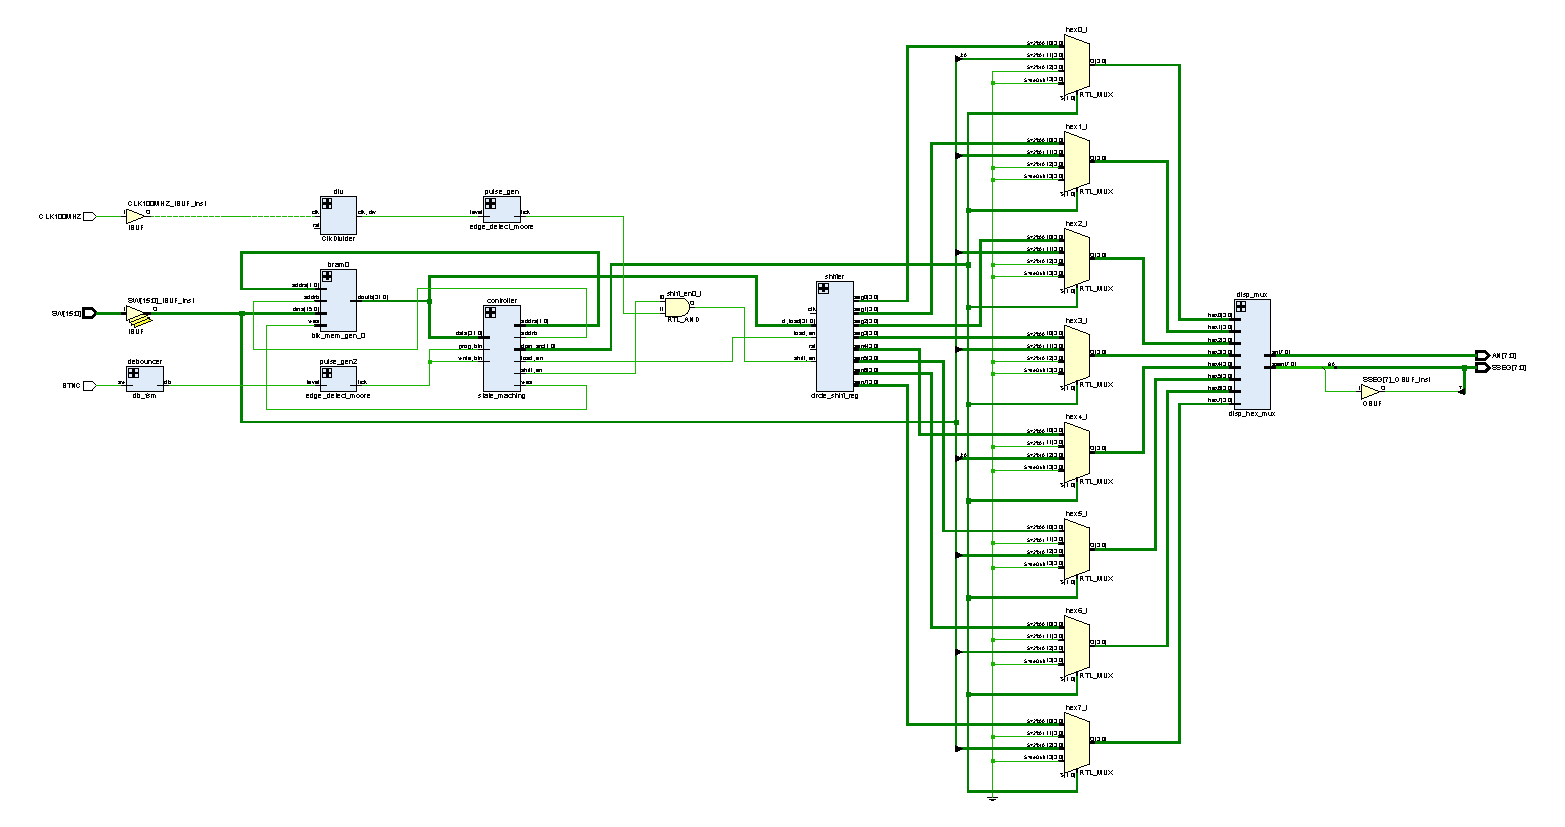
\includegraphics[trim={0.35cm 6.5cm 11cm 2.75cm},clip,width=7 in]{./figures/schematic.eps}
	\centering
	\caption{Simplified block diagram of the input and control logic.}
	\label{fig:input_logic}
\end{figure}

Figure \ref{fig:input_logic} shows the input and control logic for the system. The most important module is the controller which is comprised of a state machine that has 8 states: init, load, run, prog0, prog1, inter0, inter1, and load\_reg. 

\end{document}